\chapter{Future Work}
\label{chap:6}

Potential for future work lies in a number of fronts, both in the near term and the long term. More pressing research opportunities and improvements to the tools discussed are outlined, followed by a discussion of grander directions in which the field of image-based modeling and simulation is moving.

%%%%%%%%%%%%%%%%%%%%%%
%%%%%%%%%%%%%%%%%%%%%%
\section{Short Term}
\label{Short Term}

Tasks related to completing the full demonstration of polyhedral FEM in \textit{Celeris}, improving the image-based meshing tool \textit{Shabaka}, and improving the cardiac mechanics code \textit{Cardioid} are described herein.

\subsection[A Polyhedral Finite Element Demonstration in Cardiac \\ Mechanics]{\texorpdfstring{A Polyhedral Finite Element Demonstration in Cardiac Mechanics}{A Polyhedral Finite Element Demonstration in Cardiac Mechanics}}
\label{A Polyhedral Finite Element Demonstration in Cardiac Mechanics}

Pending some minor fixes in the Celeris codebase, the first task would be to complete the verification problems outlined in \chapref{5}. Given the accurate results provided by Imitor, it is expected that Celeris will produce satisfactory results as well. The benefit of polyhedral FEM here again is two-fold: linear element shape functions avoid the increase in DOF, and the mesh resolution is not constrained directly by the surface resolution for complex geometries. The single ventricle geometries are quite simple, but at a minimum the completion of those verification problems will show the capability to automatically generate a general polyhedral mesh and run accurate solutions while avoiding quadratic elements.

With all of the tools implemented and tested, the following step would be to run a bi-ventricular cardiac mechanics simulation to demonstrate an image-based modeling and simulation workflow using polyhedral finite elements. The highest priority is first to demonstrate capability, followed by a more direct comparison of results and computational effort when using a quadratic tet mesh in Cardioid vs. a polyhedral mesh in Celeris. This would require a convergence study in both codes to ensure that the coarsest possible meshes were being used while still attaining accurate results. This likely would also include a more comprehensive comparison of results, for example measuring stresses and strains at particular locations of interest. As of yet, there is no definitive answer to whether PFEM is a viable replacement for quadratic tetrahedra in cardiac mechanics simulations, but the preliminary theory and results look very promising.

It is worth mentioning that for PFEM to be competitive in terms of runtime, the associated code would likely need to explore an iterative solver and potentially be restructured to be able to run on a distributed memory system. There is nothing unique to PFEM that would prohibit those changes though. Depending on the degree to which the number of DOF can be reduced, and the desired simulation resolution, a direct solver on a shared memory system may well be more than sufficient. Additionally, the notion of \textit{element quality} has not yet been well defined in the context of polyhedral elements. Concepts related to mapping shape functions from the physical space to a parent space are obviously not an issue, but it is still unclear the degree to which elements near the boundary may be ``ill-shaped'' before solution accuracy begins to degrade. A complete bi-ventricular simulation would certainly clarify some of these matters.

Ultimately PFEM would exhibit its advantages most strongly in image-based biomechanics for geometries with a low surface to volume ratio, but for which a high resolution in describing the surface of the object is still desired, as well as for problems that require frequent remeshing during the simulation. It is the hope that these next steps would further solidify the promise of such an approach.

\subsection{Improvements to Image-Based Meshing Code}
\label{Improvements to Image-Based Meshing Code}

Not surprisingly, a vast number of improvements may be made to the image-based meshing code Shabaka, which would open up several additional application areas for which the code could be useful.

The highest yield improvements involve expanding capability of the interface approximation task and improving the surface reconstruction task. Interface approximation would be significantly improved if expanded to handle regions of high curvature or even sharp corners well. This would involve including additional interface ``templates'' than the plane approximation that is currently in place. Most promising additions would include a parabaloid interface, an edge interface, and a corner interface. For these interfaces, several point/normals may be placed for a single window. This extension would significantly improve the accuracy (and resulting density) of points in regions of high curvature, and allow mesh generation from images of objects with sharp edges and corners. The ability to generate high quality surfaces involving sharp features would open the door for more conventional mechanical and aerospace engineering applications.

Another important extension to the image-based meshing tool is handling multi-material image masks. As of now, the algorithm is restricted to binary image masks. Although plenty of work is still performed for single object meshes, the state of the art tools available for image-based meshing tend to have capability for multiple materials. Ideas may be gleaned from Dyadechko and Shashkov ~\cite{dyadechko_2008}, who reconstruct polygonal multi-material interfaces for Eulerian simulations of incompressible fluid flows. Although currently only applicable in two dimensions, their work provides a partitioning scheme for multiple material junctions based on similar notions of minimizing error in the moment of volume. Once the matter is sorted, Shabaka may link with the same mesh generation tools as before, which are already well-equipped to handle multi-material b-reps. This would improvement would significantly expand the range of biomedical applications, most notably to the brain and the knee (see \figref{polyknee}).

\begin{sidewaysfigure}[htbp!]
\centering
		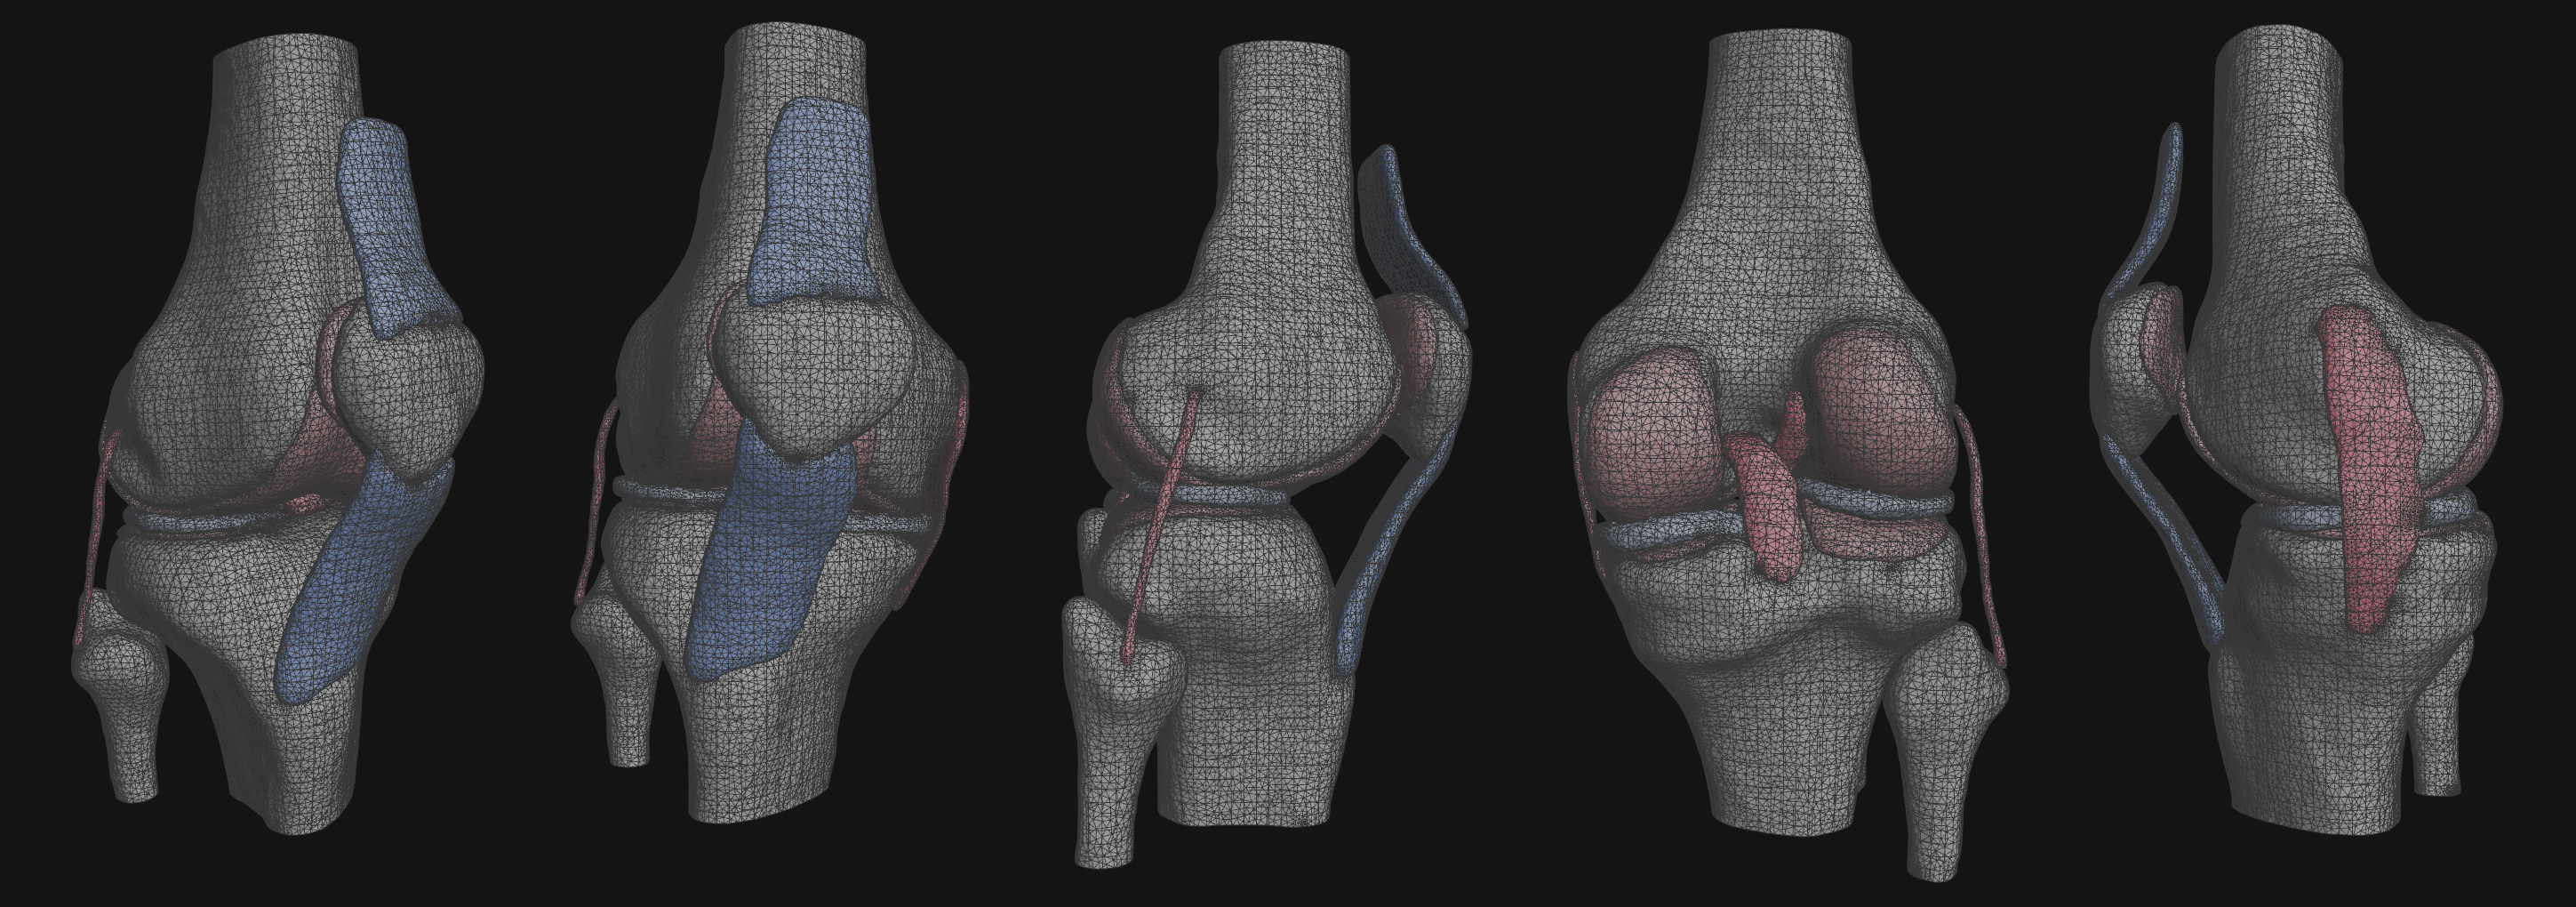
\includegraphics[width=1.0\textwidth]{media/7-polyknee/fullmesh.png}
%
\caption{Polyhedral mesh of human knee from Open Knee~\cite{erdemir_2015} b-rep}
\label{fig:polyknee}
\end{sidewaysfigure}

Improving surface reconstruction of an oriented point cloud is also critical. Work is underway within the Celeris codebase to allow for a \textit{tolerance-aware} Voronoi partioning scheme, with similar philosophy and implementation to how polyhedral meshes are constructed in that code. This could potentially mitigate the issue of ``cross-talk'' facets discussed in \chapref{3}. If a tolerance-aware approach does not resolve the issues caused by Voronoi partitions, the surface reconstruction task may be better suited to follow the approach outlined by Meyer \textit{et al.}~\cite{meyer_2008}. Provided an oriented point cloud, Meyer \textit{et al.} perform a Delaunay tetrahedralization on the point cloud itself, and then extract the surface of interest based on \textit{Delaunay} facets that share different material types.

A less urgent task would involve improving the interaction between image, image mask, and surface mesh. Work may be explored to generate point clouds directly from medical images, bypassing the image segmentation step altogether. Considering the challenge of image segmentation, this would prove to be a difficult task to produce how quality point clouds and surfaces. A more fruitful intermediate term approach may be to extract more information from the image mask in the process of generating point clouds and surfaces. For example, the underlying image carries a range of intensity values near the interface approximated by the image mask. Retaining that information with the segmented image can lead to more accurate surfaces. Indeed, Young \textit{et al.}, for example, make use of ``soft segmentations'', or what they call the \textit{partial volume effect} to produce smoother surface. In essence, they honor the fact that the image and image mask are inextricably linked.

From a software utility standpoint, the Shabaka code may be improved in some tangible ways. The bash build script should be replaced by \textit{CMake}~\cite{cmake} to download and install external packages for a more robust installation process. In the same vein, the Windows ideally would not depend on the Windows Subsystem for Linux, which is essentially a workaround for that operating system. In the interest of a faster and more reliable build, some of the dependence on fragile third-party software could be relieved by implementing some of those tools directly into Shabaka.

Finally, a necessary step in proving the quality of results from Shabaka is a numerical validation of point clouds and surface meshes for a variety of example inputs. Error measures should be defined and calculated to quantify the degree to which the interface approximations generate point clouds that honor the original surfaces from a medical image. Similarly, the quality of resulting surface meshes should be numerically measured, perhaps again comparing moments of volume between the original image mask and the resulting surface (surface area would not be a good measure, as the surface area of a voxelated mask is undesirably high compared to the underlying object in the image). Of course, these error measures ideally should be compared to other popular surface reconstruction and image-bashed meshing algorithms. Lastly, as coined by Young \textit{et al.}~\cite{young_2008}, the notion of \textit{convergence to geometry} must be further explored and understood. Specifically, mesh convergence from CAD data typically assumes there is no error in the geometric accuracy of the solid model itself. In image-based meshing, however, a finite number of sampling points are used to reconstruct the b-rep. Shabaka currently allows the user to specify the number of points to define the surface of interest, but some guidelines of how many points are actually required to ``converge to geometry'' would be quite informative and useful.

\subsection{Improvements to Cardiac Mechanics Code}
\label{Improvements to Cardiac Mechanics Code}

The cardiac mechanics code Cardioid has room for improvement and extension on several fronts as well now that a robust workflow for cardiac simulations has been established.

\cite{yang_2012, zhukov_2003}

Even without the improvements outlined here, several studies may now be performed with the available model as Cardioid moves toward answering clinical questions.

%%%%%%%%%%%%%%%%%%%%%%
%%%%%%%%%%%%%%%%%%%%%%\\
\section{Long Term}
\label{Long Term}

\subsection{Simulation of Clinical Trials}
\label{Simulation of Clinical Trials}
The problem of robust patient-specific modeling has more or less been solved, even for multi-material image masks. The next step is to combine simulation related to a particular patient with statistical and/or machine learning technologies. 
A Machine Learning System to Guide Clinical Procedures in Real-Time

\subsection[Applications in Rapid Prototyping and Additive Manufacturing]{\texorpdfstring{Applications in Rapid Prototyping and Additive \newline Manufacturing}{Applications in Rapid Prototyping and Additive \newline Manufacturing}}
\label{Applications in Rapid Prototyping and Additive Manufacturing}

\cite{fda3_2016}

\begin{sidewaysfigure}[htbp!]
\centering
		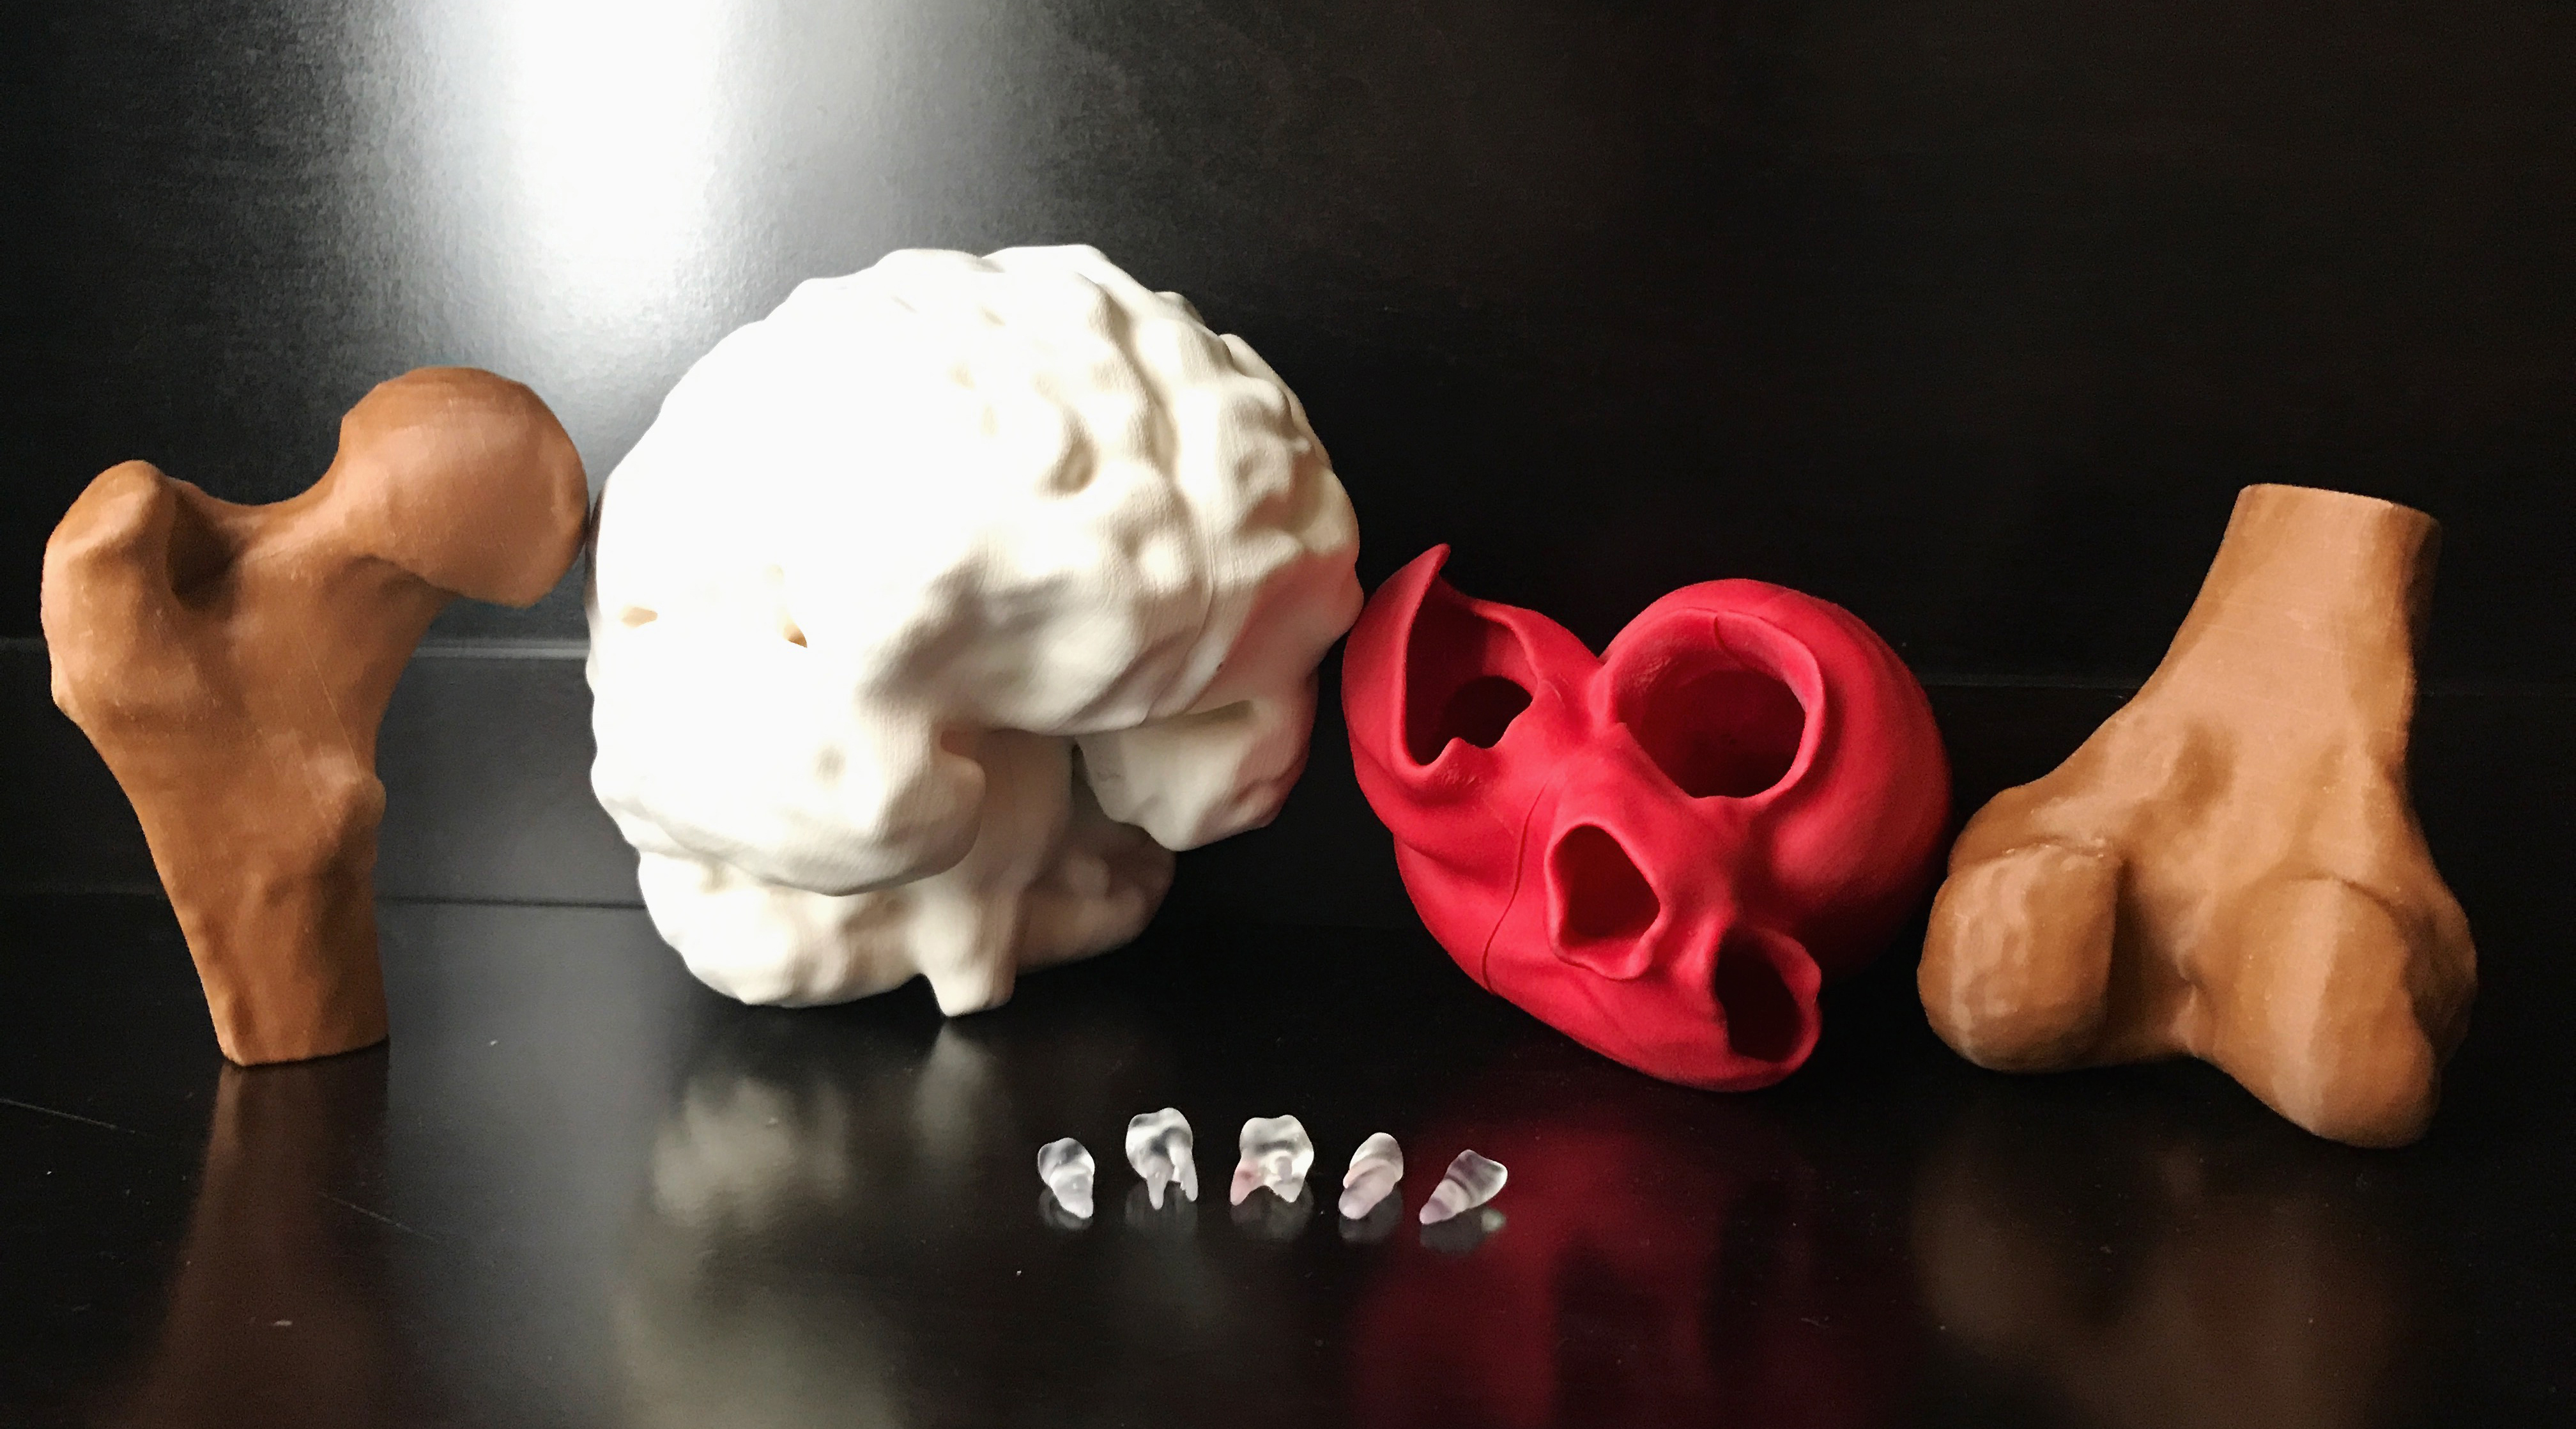
\includegraphics[width=1.0\textwidth]{media/6-3dprint/3dprint.jpg}
%
\caption{Suite of 3D-printed organs using surface meshes generated from novel image-based meshing tools}
\label{fig:3dprint}
\end{sidewaysfigure}

